\documentclass{../pi1-musterloesung}

\renewcommand{\baselinestretch}{0.998}

\begin{document}

\maketitle{8}

\section{Alles super hier (20\%)}

Es gibt nun die zwei leeren Klassen \texttt{Obstacle} und \texttt{Item}. \texttt{Wall} und \texttt{Door} erben nun von \texttt{Obstacle}, \texttt{Key} und \texttt{Bomb} von \texttt{Item}:

\lstinputlisting[firstnumber=9,firstline=9,lastline=9]{Wall.java}
\lstinputlisting[firstnumber=9,firstline=9,lastline=9]{Door.java}
\lstinputlisting[firstnumber=9,firstline=9,lastline=9]{Key.java}
\lstinputlisting[firstnumber=9,firstline=9,lastline=9]{Bomb.java}

Die Klasse \texttt{Robot} testet nun nur noch auf Kollisionen mit Hindernissen, statt direkt auf Wände oder Türen. Diese Zeile ist wegen der Bearbeitung von Aufgabe 2 nicht mehr im Quelltext enthalten:

\begin{lstlisting}[firstnumber=55]
if (getOneIntersectingObject(Obstacle.class) != null) {
\end{lstlisting}

Das \texttt{Inventory} speichert nun eine Instanz von \texttt{Item}:

\lstinputlisting[firstnumber=12,firstline=12,lastline=12]{Inventory.java}
\lstinputlisting[firstnumber=25,firstline=25,lastline=25]{Inventory.java}
\lstinputlisting[firstnumber=45,firstline=45,lastline=45]{Inventory.java}

Die Klasse \texttt{Robot} hebt nun \texttt{Item}s auf (auch nicht mehr vorhanden):

\begin{lstlisting}[firstnumber=152]
                Item object = (Item) getOneIntersectingObject(Item.class);
\end{lstlisting}

\paragraph{Tests.} Der Roboter bleibt immer noch vor Wänden und Türen stehen. Schlüssel und Bomben können weiterhin aufgehoben und abgelegt werden. Mit dem Schlüssel können immer noch Türen geöffnet und mit der Bombe Wände gesprengt werden.

\section{Massenkarambolage (30\%)}
\label{s:collider}

\emph{Führt eine Superklasse für alle Klassen ein, die auf Kollisionen testen.}

\lstinputlisting[firstnumber=13,firstline=13,lastline=14]{Collider.java}
\lstinputlisting[firstnumber=162,firstline=162,lastline=162]{Collider.java}

1) \emph{Eine Methode, die das Objekt einer bestimmten Klasse zurückliefert, mit dem gerade eine Kollision besteht, bzw. \texttt{null}, wenn keine Kollision besteht. Vorerst ist diese Methode einfach nur ein Synonym für \texttt{getOneIntersectingObject}.} (Zeile 33 ist wegen Aufgabe 3 nicht mehr vorhanden):

\begin{lstlisting}[firstnumber=31]
    public Actor getCollidingObject(Class clazz)
    {
        return getOneIntersectingObject(clazz);
    }
\end{lstlisting}

2) \emph{Eine Komfortmethode, die zurückliefert, \emph{ob} gerade eine Kollision mit einem Objekt einer bestimmten Klasse besteht. Sie soll sich auf die erste Methode abstützen.}

\lstinputlisting[firstnumber=49,firstline=49,lastline=52]{Collider.java}

3) \emph{Eine Methode, die zurückliefert, ob gerade eine neue Kollision mit einer Instanz einer bestimmten Klassen begonnen hat. Da diese Methode für verschiedene Klassen aufgerufen werden kann, muss sie darüber Buch führen, ob und wenn ja, mit welcher Instanz einer Klasse gerade eine Kollision besteht. So kann sie auch zurückliefern, wenn plötzlich mit einer anderen Instanz derselben Klasse eine Kollision begonnen hat. Auch diese Methode soll sich auf die erste Methode abstützen.}

Der aktuelle Kollisionszustand wird pro Klasse in einer \texttt{HashMap} gespeichert. Der Einfachheit halber wird auch der Wert \texttt{null} in der \texttt{HashMap} abgelegt, wenn es gerade keine Kollision gibt. Eine neue Kollision liegt immer vor, wenn wir uns gerade in einer Kollision befinden und das Objekt ein anderes ist als zuvor, wobei dies auch den Fall einschließt, dass wir zuvor keine Kollision hatten:

\lstinputlisting[firstnumber=21,firstline=21,lastline=22]{Collider.java}
\lstinputlisting[firstnumber=61,firstline=61,lastline=68]{Collider.java}

\emph{Baut alle Kollisionstests in eurem Code so um, dass sie nur noch diese drei Methoden benutzen.}

Die Klassen \texttt{Robot}, \texttt{Exit}, \texttt{Smiley} und \texttt{Skull} erben nun von \texttt{Collider}. In diesen Klassen wurde, wenn vorhanden, auch das Attribut \texttt{intersecting} entfernt, weil es nicht mehr benötigt wird:

\lstinputlisting[firstnumber=9,firstline=9,lastline=9]{Robot.java}
\lstinputlisting[firstnumber=9,firstline=9,lastline=9]{Exit.java}
\lstinputlisting[firstnumber=9,firstline=9,lastline=9]{Smiley.java}
\lstinputlisting[firstnumber=9,firstline=9,lastline=9]{Skull.java}

In der Klasse \texttt{Robot} führen die Methoden \texttt{act}, \texttt{countCollisions}, \texttt{unlockDoor}, \texttt{blowUpObstacle} und \texttt{pickUpOrDropObject} Kollisionstests durch:

\lstinputlisting[firstnumber=52,firstline=50,lastline=50]{Robot.java}
\lstinputlisting[firstnumber=89,firstline=89,lastline=91]{Robot.java}
\lstinputlisting[firstnumber=117,firstline=117,lastline=120]{Robot.java}
\lstinputlisting[firstnumber=131,firstline=131,lastline=133]{Robot.java}
\lstinputlisting[firstnumber=150,firstline=150,lastline=151]{Robot.java}

In den Klassen \texttt{Exit}, \texttt{Smiley} und \texttt{Skull} sind nur die Methoden \texttt{act} vom Umbau betroffen:

\lstinputlisting[firstnumber=38,firstline=38,lastline=40]{Exit.java}
\lstinputlisting[firstnumber=18,firstline=18,lastline=18]{Smiley.java}
\lstinputlisting[firstnumber=18,firstline=18,lastline=18]{Skull.java}

\paragraph{Tests.} Grundsätzlich werden alle Kollisionen erkannt, die vor dem Umbau auch bereits erkannt wurden, d.h. der Roboter kann sich nicht durch Hindernisse bewegen, kann weiterhin Schlüssel und Bombe aufnehmen, Berührungen mit Smileys lassen den Spielstand um 10 Punkte wachsen und eine Berührung des Totenschädels beendet das Spiel. Ebenso spielen Smileys und Totenschädel weiterhin ihren Sound ab und der Ausgang schaltet den Level um. Zusätzlich kann man aber auch mehrere Smileys dicht nebeneinander platzieren und mit dem Roboter immer zwischen ihnen hin und herfahren. Obwohl der Roboter dabei immer mindestens einen der Smileys berührt, wächst der Punktestand dennoch bei jedem Wechsel von einem Smiley zum nächsten, d.h. es wird erkannt, dass das Objekt, mit dem der Roboter kollidiert, gewechselt hat. Platziert man Smiley und Totenschädel dicht beieinander, kann man auch testen, dass trotz einer andauernden Kollision mit einem Smiley sofort festgestellt wird, wenn der Totenschädel berührt wird.

\section{Richtig kollidieren (50\%)}

1) \emph{Erweitert die erste Methode aus \ref{s:collider} so, dass sie die Liste aller Schnittobjekte durchläuft, d.h. die Rückgabe von \texttt{getIntersectingObjects} verarbeitet. Erst, wenn für eines der Objekte bestätigt wird, dass wirklich eine Kollision besteht, wird dieses als Ergebnis zurückgeliefert. Besteht zu keinem Objekt eine Kollision, ist die Rückgabe weiterhin \texttt{null}.}

\lstinputlisting[firstnumber=31,firstline=31,lastline=33]{Collider.java}
\lstinputlisting[firstnumber=35,firstline=35,lastline=41]{Collider.java}

2) \emph{Um festzustellen, ob tatsächlich eine Kollision besteht, muss für jedes nicht-transparente Pixel des einen Objekts (z.B. jenem, das den Kollisionstest durchführt) überprüft werden, ob sich an derselben Stelle (in Weltkoordinaten) in dem anderen Objekt auch ein nicht-transparentes Pixel befindet. Sobald dies der Fall ist, gibt es tatsächlich eine Kollision. Um dies herauszubekommen, müssen die Pixelkoordinaten des Bildes des ersten Objekts in Weltkoordinaten umgerechnet werden und von dort weiter in Pixelkoordinaten des Bildes des zweiten Objekts.}

\lstinputlisting[firstnumber=78,firstline=78,lastline=79]{Collider.java}
\lstinputlisting[firstnumber=82,firstline=82,lastline=89]{Collider.java}
\lstinputlisting[firstnumber=93,firstline=93,lastline=93]{Collider.java}
\lstinputlisting[firstnumber=95,firstline=95,lastline=134]{Collider.java}

3) \emph{Da man bei den Transformationen viel falsch machen kann, baut ihr einen Testmodus ein. Ist dieser aktiv, werden überhaupt keine Kollisionen mehr gemeldet. Stattdessen werden im Bild des Actors, der auf Kollisionen testet, alle Pixel farblich markiert, die mit einem anderen Objekt kollidieren, z.B. in \texttt{Color.RED}.}

\lstinputlisting[firstnumber=15,firstline=15,lastline=19]{Collider.java}
\lstinputlisting[firstnumber=34,firstline=34,lastline=34]{Collider.java}
\lstinputlisting[firstnumber=80,firstline=80,lastline=80]{Collider.java}
\lstinputlisting[firstnumber=90,firstline=90,lastline=94]{Collider.java}
\lstinputlisting[firstnumber=136,firstline=136,lastline=161]{Collider.java}

\paragraph{Tests.} Der Roboter kann nun deutlich dichter an andere Objekte heranfahren, z.B. kann er die Ecke einer Wand mit seinen zwei Strahlern auch umschließen (siehe Abb.~\ref{f:screenshots} links).  Dies ist nicht immer offensichtlich, da er sich ja mit einer Schrittweite von fünf durch die Welt bewegt und deshalb manchmal immer noch in größeren Abständen von Objekten zum Stehen kommt. Mit aktiviertem Testmodus kann man sehen, dass die überlappenden Teile rot eingefärbt werden. Um diesen Test mit beliebigen Rotationen beider an einer Kollision beteiligten Objekten durchführen zu können, drehen sich die Totenschädel nun langsam, so dass man den sich drehenden Roboter mit einem sich drehenden Totenschädel überlappen lassen kann (siehe Abb.~\ref{f:screenshots} rechts).

\begin{figure}[h]
\centering
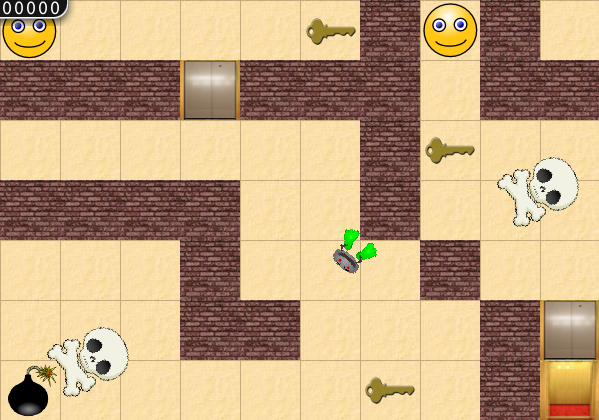
\includegraphics[width=0.495\textwidth]{wallcollision.png}
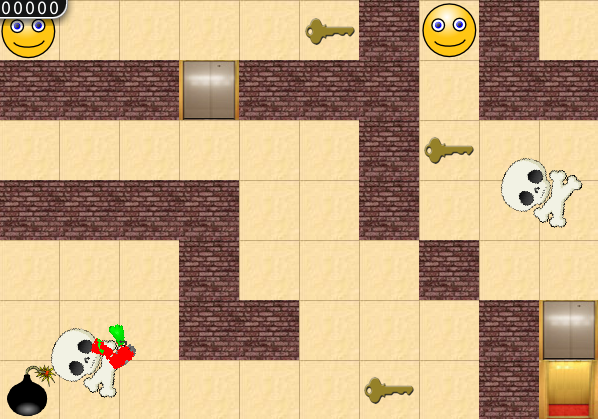
\includegraphics[width=0.495\textwidth]{skullcollision.png}
\caption{Kollision mit einer Wand bei deaktiviertem Testmodus und Überlappung mit einem Totenschädel (in rot) bei aktiviertem Testmodus}
\label{f:screenshots}
\end{figure}

\end{document}